% !TEX program = xelatex
%% Requires compilation with XeLaTeX or LuaLaTeX
\documentclass[10pt,xcolor={table,dvipsnames},t]{beamer}
\usepackage{biblatex}
\usepackage{caption}
\setbeamertemplate{caption}[numbered]
\addbibresource{reference.bib}
\usepackage{hyperref}
\hypersetup{ 
pdfpagemode=FullScreen,  
colorlinks=true,linkcolor=blue}
\usepackage{enumerate}
\usepackage{algorithm}
\usepackage{algpseudocode}
\usepackage{listings}
\usepackage{xcolor}
\usepackage{graphicx}

\definecolor{codegreen}{rgb}{0,0.6,0}
\definecolor{codegray}{rgb}{0.5,0.5,0.5}
\definecolor{codepurple}{rgb}{0.58,0,0.82}
\definecolor{backcolour}{rgb}{0.95,0.95,0.92}

\lstdefinestyle{mystyle}{
    backgroundcolor=\color{backcolour},   
    commentstyle=\color{codegreen},
    keywordstyle=\color{magenta},
    numberstyle=\tiny\color{codegray},
    stringstyle=\color{codepurple},
    basicstyle=\ttfamily\footnotesize,
    breakatwhitespace=false,         
    breaklines=true,                 
    captionpos=b,                    
    keepspaces=true,                 
    numbers=left,                    
    numbersep=5pt,                  
    showspaces=false,                
    showstringspaces=false,
    showtabs=false,                  
    tabsize=2
}

\lstset{style=mystyle}

% Flow chart config
\usepackage{tikz}
\usetikzlibrary{calc,trees,positioning,arrows,fit,shapes,calc,tikzmark,matrix}
\usepackage{eso-pic}
\usetikzlibrary{shapes.geometric, arrows}
\tikzstyle{startstop} = [rectangle, rounded corners, minimum width=3cm, minimum height=1cm,text centered, draw=black, fill=red!30]
\tikzstyle{io} = [trapezium, trapezium left angle=70, trapezium right angle=110, minimum width=3cm, minimum height=1cm, text centered, draw=black, fill=blue!30]
\tikzstyle{process} = [rectangle, minimum width=3cm, minimum height=1cm, text centered, draw=black, fill=orange!30]
\tikzstyle{decision} = [diamond, minimum width=3cm, minimum height=1cm, text centered, draw=black, fill=green!30]
\tikzstyle{arrow} = [thick,->,>=stealth]

\usetheme{UCBerkeley}

\title[Your Short Title]{STMC Coding Team Training}
\subtitle{Lesson 8: Introduction to AI, ML and their applications}
\author{Tsai Yun Chen}
%\institute{}
\date{\today}

\begin{document}

\begin{frame}
  \titlepage
\end{frame}

% Uncomment these lines for an automatically generated outline.
%\begin{frame}{Outline}
%  \tableofcontents
%\end{frame}

\section{Class Goal}

\begin{frame}{Goal today}
Today we will briefly talk about the history, development and concept of AI, the definition and examples of Machine Learning Model, we will try out two different state-of-the-art ML models.
\begin{itemize}
  \item What is AI?
  \item A brief history timeline of AI
  \item Overview of ML
  \item ML model 1: Stable Diffusion
  \item ML model 2: GPT-4
  \item What's in the future?
\end{itemize}
\end{frame}

\begin{frame}{What is AI?}
  \begin{columns}
    \begin{column}[T]{0.6\textwidth}
      \begin{itemize}
        \item Artificial Intelligence (AI)
        \item Alan Turing, the father of Theoretical Computer Science and AI
        \item Central Question: Can machine think and behave like a human?
        \item In 1950s, the field of study in AI was founded
      \end{itemize}
    \end{column}
    \begin{column}[T]{0.4\textwidth}
      \begin{figure}
        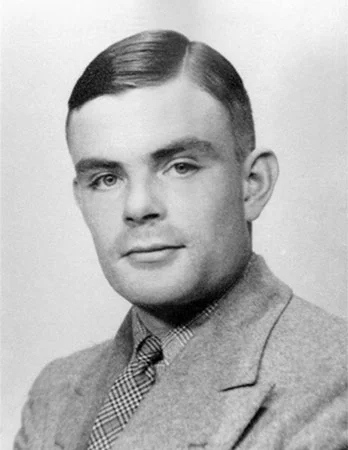
\includegraphics[width=0.6\textwidth]{img/Alan-Turing.png}
        \caption{retrieved from: \href{https://www.britannica.com/biography/Alan-Turing}{Alan Turing, B.J. Copeland}}
      \end{figure}
    \end{column}
  \end{columns}
\end{frame}

\begin{frame}{First and Second AI Winter}
  \begin{itemize}
    \item In late 1970s, development in AI slow down
    \item Reasons:
    \begin{itemize}
      \item Computational Power
      \item Lack of Framework
    \end{itemize}
    \item In the 1980s, Expert System is proposed
    \item It failed due to similar reasons
  \end{itemize}
  \begin{figure}
    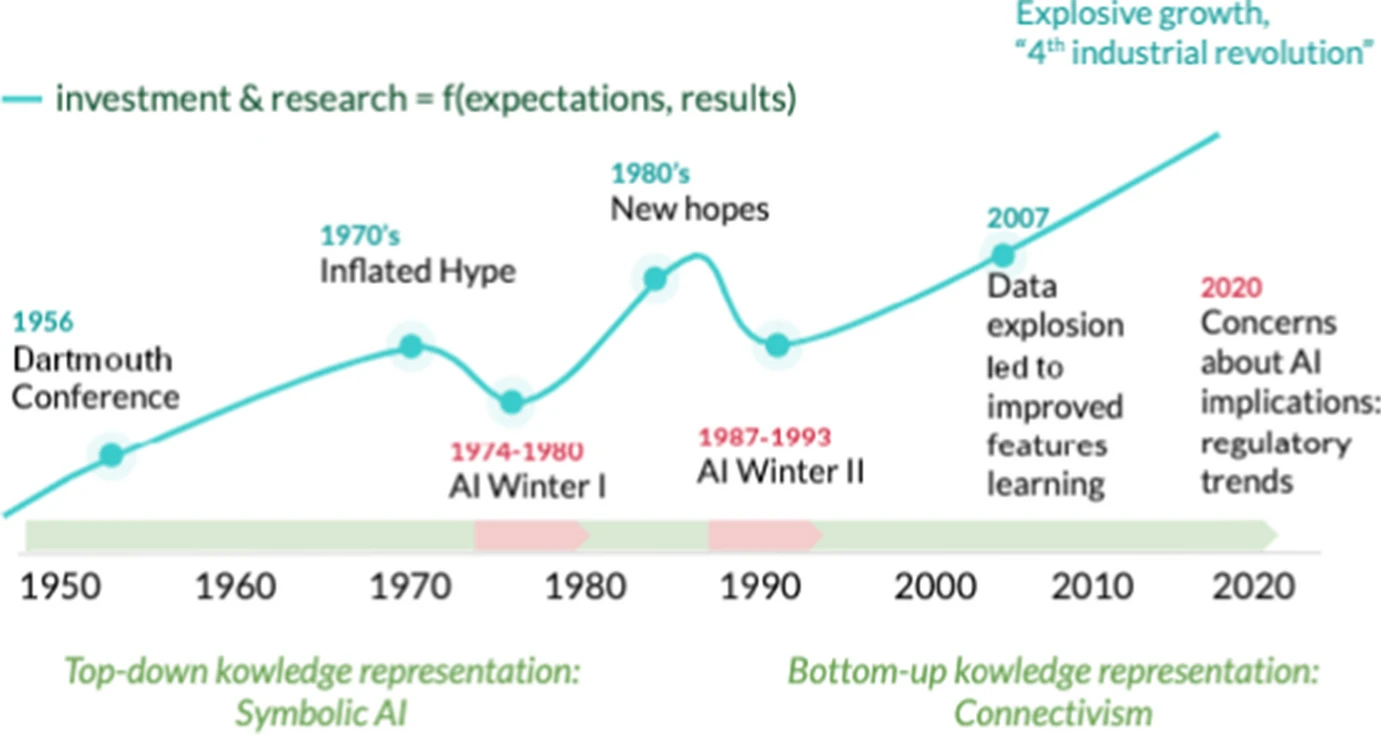
\includegraphics[width=0.6\textwidth]{img/AIwinter.png}
    \caption{\textcolor{white}{retrieved from: } \href{https://link.springer.com/article/10.1007/s10506-022-09309-8}{The winter, the summer and the summer dream of artificial intelligence in law, Enrico Francesconi}}
  \end{figure}
\end{frame}

\begin{frame}{Rise of Machine Learning}
  \begin{itemize}
    \item The concept of Machine Learning was raised in 1960s
    \item Central Question: Can machine learn knowledge like a human?
    \item But... How do we define learn? How do we prove we learnt something?
    \item We need a bit Mathematics to help with that
  \end{itemize}
\end{frame}

\begin{frame}{Function: Pattern of numbers}
  \begin{itemize}
    \item Imagine we are learning about the concept of even number
    \item It contains a set of numbers, $\{2,4,6,8,...\}$
    \item But to the machine, it is just a bunch of numbers...
    \item Pattern is the key!
    \item (mathematic) function is good for capturing pattern of numbers
    \item In this example, they all lies on the line $y=2x$
  \end{itemize}
\end{frame}

\begin{frame}{Regression}
  \begin{columns}
    \begin{column}[T]{0.6\textwidth}
      \begin{itemize}
        \item In general, consider you have a bunch of data
        \item The way we \texttt{learn} the data is by finding a (good) function that contain all the points
        \item But... There may not always exist such a function
        \item To make our life easier, we accept the function that is \texttt{close} too most of the data points
        \item Such technique is called Regression
      \end{itemize}
    \end{column}
    \begin{column}[T]{0.4\textwidth}
      \begin{figure}
        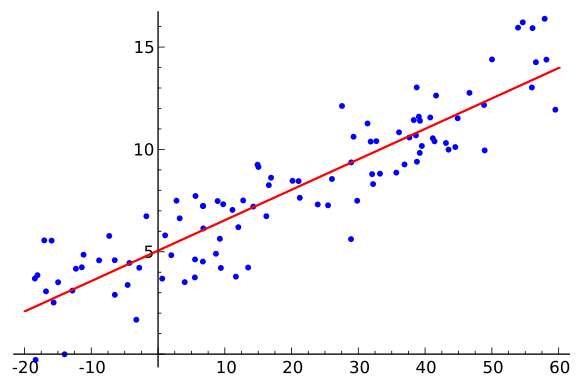
\includegraphics[width=0.8\textwidth]{img/Linear_regression.png}
        \caption{retrieved from: \href{https://en.wikipedia.org/wiki/Regression_analysis}{Regression analysis, Wikipedia}}
      \end{figure}
    \end{column}
  \end{columns}
\end{frame}

\begin{frame}{Artificial Neural Network (ANN)}
  \begin{columns}
    \begin{column}[T]{0.6\textwidth}
      \begin{itemize}
        \item Regression is good, but there's a problem\dots
        \item How do I know a function is good for my data?
        \item We need a more general way of representing function
        \item Neural Network is all you need!
        \item A Neural Network consist of\dots
        \begin{itemize}
          \item Input Layers
          \item Zero or more Hidden Layers
          \item Output Layers
        \end{itemize}
        \item Most of the function can be approximated as a Neural Network
      \end{itemize}
    \end{column}
    \begin{column}[T]{0.4\textwidth}
      \begin{figure}
        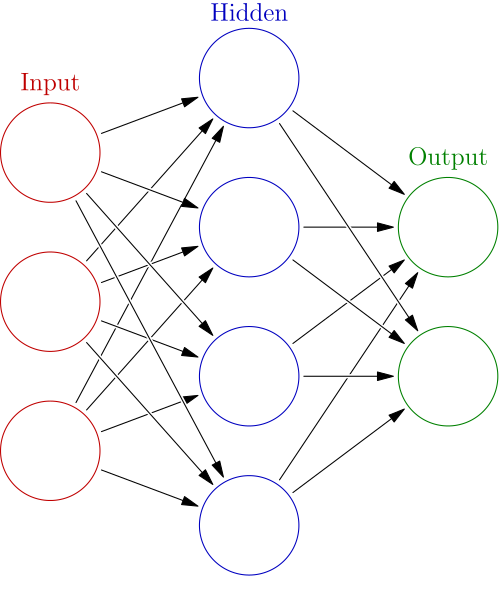
\includegraphics[width=0.8\textwidth]{img/Colored_neural_network.png}
        \caption{retrieved from: \href{https://en.wikipedia.org/wiki/Neural_network_(machine_learning)}{Neural network (machine learning), Wikipedia}}
      \end{figure}
    \end{column}
  \end{columns}
\end{frame}

\begin{frame}{Learning, Training and Testing}
  \begin{itemize}
    \item Just like we have exam in schools
    \item We let the function we learnt to do a test to see how close is it to our data set
    \item This process is called testing
    \item Training refers to the process of feeding in data to find the good function we need
    \item Usually we separate data into training set and testing set
    \item The process of training, testing and fine-tuning is how we conduct Machine Learning (usually)
  \end{itemize}
\end{frame}

\begin{frame}{Deep Learning}
  \begin{columns}
    \begin{column}[T]{0.6\textwidth}
      \begin{itemize}
        \item the technique to use multiple hidden layers for constructing complicated function
        \item Since numbers of layers increase, parameter increase as well
        \item We need a really large data set to find out which function we need
      \end{itemize}
    \end{column}
    \begin{column}[T]{0.4\textwidth}
      \begin{figure}
        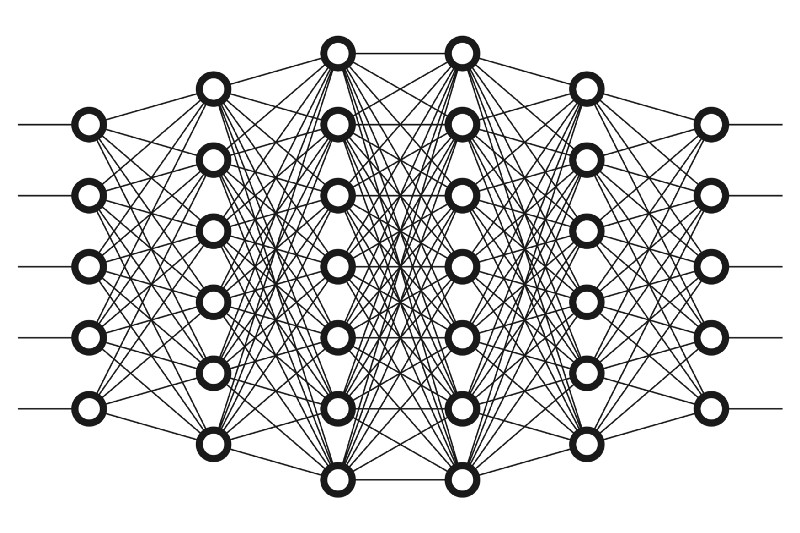
\includegraphics[width=0.8\textwidth]{img/DeepLearning.jpeg}
        \caption{retrieved from: \href{https://www.freecodecamp.org/news/want-to-know-how-deep-learning-works-heres-a-quick-guide-for-everyone-1aedeca88076/}{Want to know how Deep Learning works? Here’s a quick guide for everyone, Radu Raicea}}
      \end{figure}
    \end{column}
  \end{columns}
\end{frame}

\begin{frame}{Sounds simple?}
  \begin{itemize}
    \item The above is an \textbf{extremely} simplified introduction to AI and ML
    \item As you can imagine, tons of math lies underneath are omitted
    \item A lot of scientists are still working hard to improve different kind of model/methods
    \item Let's try some really cool tools people developed
  \end{itemize}
  \begin{figure}
    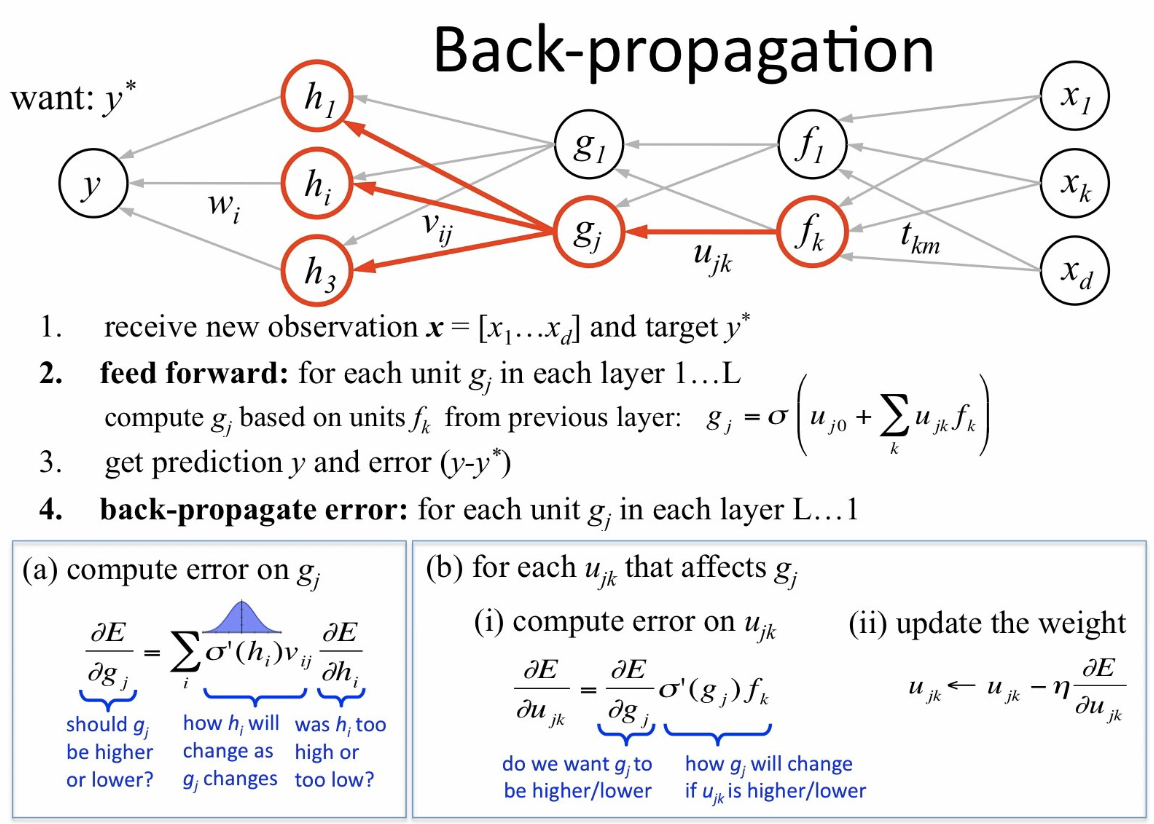
\includegraphics[width=0.6\textwidth]{img/BackPropagation.png}
    \caption{\textcolor{white}{retrieved from:} \href{https://medium.com/@jorgesleonel/backpropagation-cc81e9c772fd}{Backpropagation, Jorge Leonel}}
  \end{figure}
\end{frame}

\begin{frame}{Stable Diffusion}
  \begin{itemize}
    \item A model that generate Images according to the text describing it
    \item Proposed by CompVis group at LMU M\"{u}nich in 2022
    \item Let's try to generate a few images with your own prompt first!
    \item Make sure the preprocessing part is done.
    \item Modify the string \texttt{prompt} to generate a image you want
    \item Do you spot any unusual part in the generated image?
    \item Can you modify the prompt to fix it?
  \end{itemize}
\end{frame}

\begin{frame}{Exercise}
  \begin{itemize}
    \item Modify the code so that it asked user for a input and try to generate a image for the input
    \item To make it more interative, after the image is generated, ask the user whether he/she want to generate another one
    \item Modify the code so that it generated multiple images and compare them
    \item Let the user to choose which image to save
  \end{itemize}
\end{frame}

\begin{frame}{GPT-4}
  \begin{itemize}
    \item A model that generate text-response according to the text input provided
    \item Proposed by OpenAi in 2023
    \item Let's try to Talk with the model, ask it a few questions
    \item The reaction might be slow, be patient with it
  \end{itemize}
\end{frame}

\begin{frame}{What's in the future?}
  \begin{itemize}
    \item Make GPT even smarter
    \item Application to other area: robotics, vehicle, medical-use...
    \item Small-Data AI, customized AI
    \item Quantum-based technology
  \end{itemize}
\end{frame}
\end{document}
